
\documentclass[a4paper, 12pt]{article}
\usepackage[T1]{fontenc}
\usepackage{times}
\usepackage[swedish]{babel}
\usepackage[utf8]{inputenc}
%\usepackage{dtklogos}
\usepackage{wallpaper}
\usepackage[absolute]{textpos}
\usepackage[top=2cm, bottom=2.5cm, left=3cm, right=3cm]{geometry}
\usepackage{appendix}
\usepackage[nottoc]{tocbibind}
\setcounter{secnumdepth}{3}
\setcounter{tocdepth}{3}
\usepackage{sectsty}
\sectionfont{\fontsize{14}{15}\selectfont}
\subsectionfont{\fontsize{12}{15}\selectfont}
\subsubsectionfont{\fontsize{12}{15}\selectfont}
\usepackage{csquotes} 
\renewcommand{\thetable}{\arabic{section}.\arabic{table}}  
\renewcommand{\thefigure}{\arabic{section}.\arabic{figure}} 
\usepackage{amsmath}
\usepackage{algorithm}
\usepackage[noend]{algpseudocode}

\usepackage{listings}
\lstset{defaultdialect=[x86masm]Assembler}


\newsavebox{\mybox}
\newlength{\mydepth}
\newlength{\myheight}
\newenvironment{sidebar}
{\begin{lrbox}{\mybox}\begin{minipage}{\textwidth}}
{\end{minipage}\end{lrbox}
 \settodepth{\mydepth}{\usebox{\mybox}}
 \settoheight{\myheight}{\usebox{\mybox}}
 \addtolength{\myheight}{\mydepth}
 \noindent\makebox[0pt]{\hspace{-20pt}\rule[-\mydepth]{1pt}{\myheight}}
 \usebox{\mybox}}

\newcommand\BackgroundPic{
    \put(-2,-3){
    
\includegraphics[keepaspectratio,scale=0.3]{lnu_etch.png} 
    }
}
\newcommand\BackgroundPicLogo{
    \put(30,740){
	
\includegraphics[keepaspectratio,scale=0.10]{logo.png}     
    }
}


%\usepackage[backend=bibtex,bibencoding=ascii,style=authoryear,sorting=none]{biblatex}

\title{	
\vspace{-8cm}
\begin{sidebar}
    \vspace{5cm}
    \normalfont \normalsize
    \Huge Rapport \\
    \vspace{-1.3cm}
\end{sidebar}
\vspace{3cm}
\begin{flushleft}
    \huge Laboratory Report\\  
\end{flushleft}
\null
\vfill
\begin{textblock}{6}(10,13)
\begin{flushright}
\begin{minipage}{\textwidth}
\begin{flushleft} \large
	\emph{Author:} Caroline Nilsson \\ Daniel Alm Grundström \\
	%\emph{Handledare:} \\ 
	\emph{Termin:} HT 2017\\ 
	\emph{Course:} 1DT301 - Computer Technology I\\
\end{flushleft}
\end{minipage}
\end{flushright}
\end{textblock}
}
\date{\today} 



\begin{document}

\pagenumbering{gobble}
\newgeometry{left=5cm}
\AddToShipoutPicture*{\BackgroundPic}
\AddToShipoutPicture*{\BackgroundPicLogo}
\maketitle
\restoregeometry
\clearpage



\pagenumbering{gobble}

\tableofcontents
\newpage
\pagenumbering{arabic}



\section{Introduktion}
In the process of working with the laboratory assignments we started by doing research about the assembly language and the STK600 in order to better understand how to solve the different assignments. 
In each assignment we first created a pseudocode solution which we converted to flowchart diagrams, then it was rather simple to convert this into assembly language. Common for all assignments is also that we have been using the simulations to confirm that the program is working and completing the correct tasks. 

\newpage
\section{Assignment 1 - Light LED2}
In the first assignment we were to light up LED2 (which is the third light counting from the right). 

\begin{algorithm}
\begin{algorithmic}
\Procedure{Pseudocode}{}
\State{$PortB = output$}
\Repeat
\State{$Led2\ bitstring \rightarrow PortB$}
\Until{$\infty$}
\EndProcedure
\caption{Light LED2}
\label{assign1.pseudo}
\end{algorithmic}
\end{algorithm}

\begin{figure}[h]
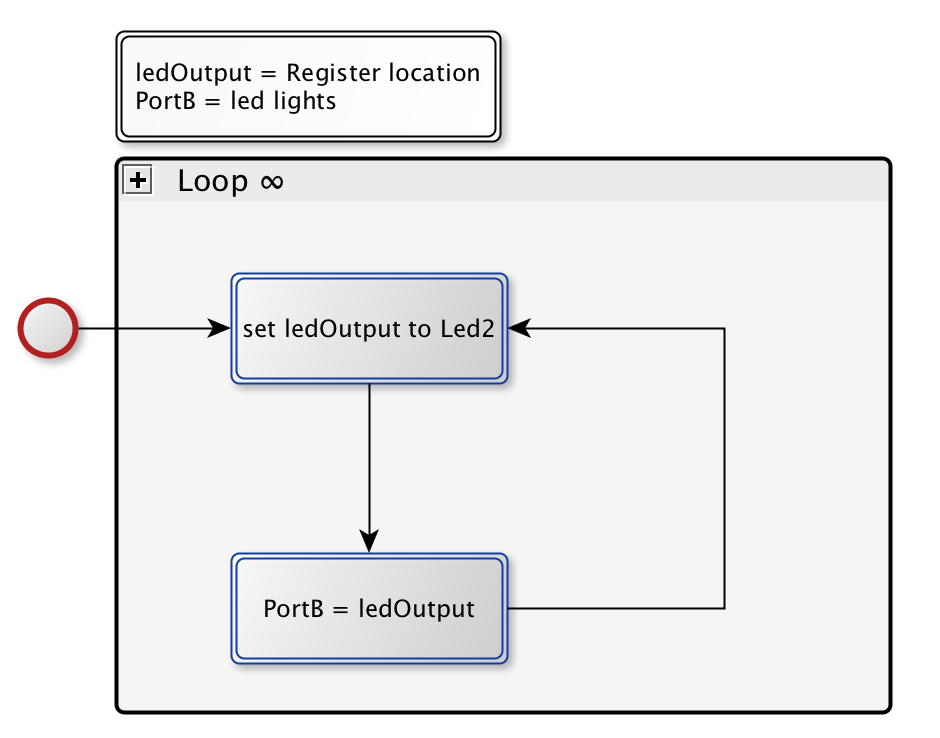
\includegraphics[scale=0.5]{Flowchart_pics/assignment1_pic.png} 
\caption{Flowchart}
\label{assign1.flow}
\end{figure}

The pseudocode (see algorithm \ref{assign1.pseudo}) and the flowchart (see figure \ref{assign1.flow}) shows that we first set Port B as an output port, the value 0000 0100 is saved at a register location (in our case that is R16) and then sent to Port B which makes LED2 (or the third led from the right) light up. 
Minimum lines of code?
\newpage
\subsection{Assembly Program}
\begin{lstlisting}[basicstyle=\tiny]
;>>>>>>>>>>>>>>>>>>>>>>>>>>>>>>>>>>>>>>>>>>>>>>>>>>>>>>>>>>>
;   1DT301, Computer Technology I
;   Date: 2017-09-02
;   Author:
;                       Caroline Nilsson            (cn222nd)
;                       Daniel Alm Grundstrom       (dg222dw)
;
;   Lab number:         1
;   Title:              How to use the PORTs. Digital input /output.
;                       Subroutine call.
;
;   Hardware:           STK600, CPU ATmega2560
;
;   Function:           Lights LED2 on PORTB
;
;   Input ports:        N/A
;
;   Output ports:       PIN2 on PORTB
;
;   Subroutines:        N/A
;   Included files:     m2560def.inc
;
;   Other information:
;
;   Changes in program: 
;                       2017-09-01:
;                       Implemented flowchart design.
;
;                       2017-09-02:
;                       Added comments and .def for r16
;
;<<<<<<<<<<<<<<<<<<<<<<<<<<<<<<<<<<<<<<<<<<<<<<<<<<<<<<<<<<<
.include "m2560def.inc"
.def ledOutput = r16

; Set PORTB to output
ldi ledOutput, PINB2
out DDRB, ledOutput

; TODO: Test on hardware if it is neccessary to have this in a loop
loop:
    out PORTB, ledOutput        ; Turn on LED2 on PORTB
    rjmp loop


\end{lstlisting}

\newpage

\section{Assignment 2 - Switch light corresponding LED}
\begin{algorithm}
\begin{algorithmic}
\Procedure{Pseudocode}{}
\State{$PortB = output$}
\State{$PortD = input$}
\Repeat
\State{$PortD\ value \rightarrow switchState$} \Comment{$switchState = register\ location$}
\State{$Invert\ value\ at\ switchState$}
\State{$switchState \rightarrow PortB$}
\Until{$\infty$}
\EndProcedure
\caption{Switches pressed lights corresponding LED}
\label{assign2.pseudo}
\end{algorithmic}
\end{algorithm}

\begin{figure}[h]
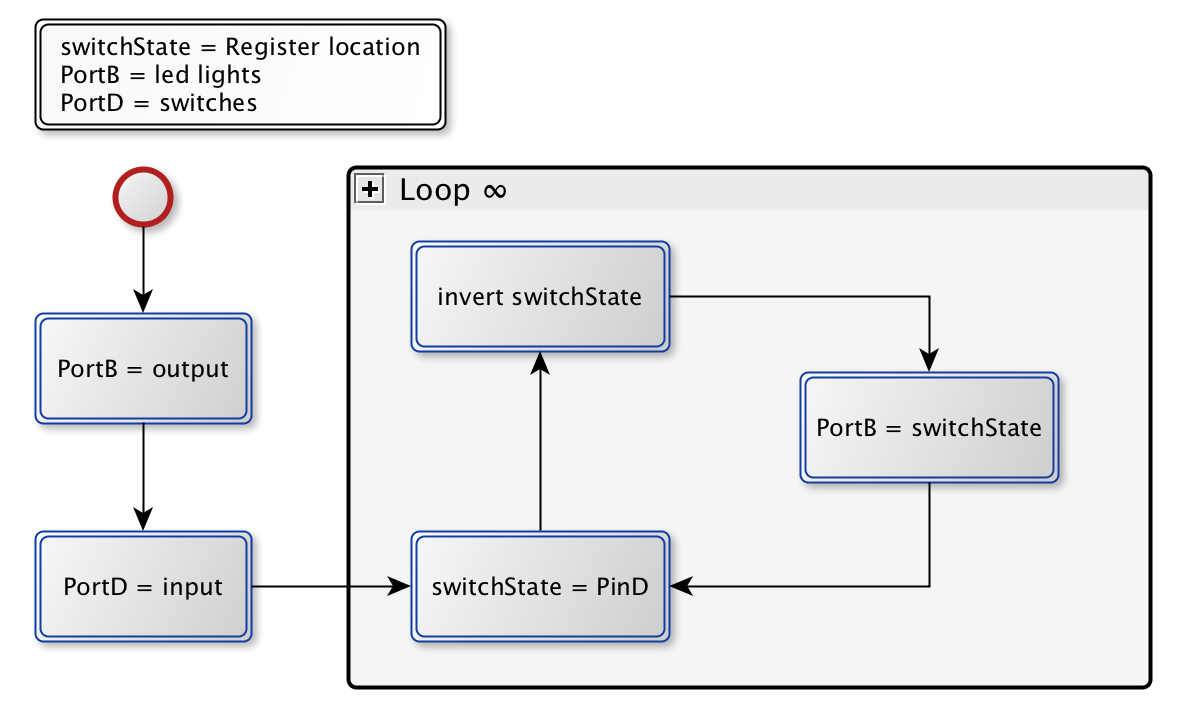
\includegraphics[scale=0.5]{Flowchart_pics/assignment2_pic.png} 
\caption{Basic flow in order to read switches and light corresponding LED}
\label{assign2.flow}
\end{figure}
\newpage
\subsection{Assembly Program}
\begin{lstlisting}[basicstyle=\tiny]
;>>>>>>>>>>>>>>>>>>>>>>>>>>>>>>>>>>>>>>>>>>>>>>>>>>>>>>>>>>>
;   1DT301, Computer Technology I
;   Date: 2017-09-02
;   Author:
;                       Caroline Nilsson            (cn222nd)
;                       Daniel Alm Grundstrom       (dg222dw)
;
;   Lab number:         1
;   Title:              How to use the PORTs. Digital input /output.
;                       Subroutine call.
;
;   Hardware:           STK600, CPU ATmega2560
;
;   Function:           Reads input from the switches SW0..SW7 and lights the
;                       corresponding LED when a switch is pressed. (SW0 lights
;                       LED0, SW1 lights LED1 and so on)
;
;   Input ports:        PORTD
;
;   Output ports:       PORTB
;
;   Subroutines:        N/A
;   Included files:     m2560def.inc
;
;   Other information:  Since a pressed switch is registered as a 0 and a
;                       released switch is registered as a 1. The bit string
;                       read from PORTD must be inverted before the output
;                       is redirected to the LEDs.
;
;   Changes in program: 
;                       2017-09-01:
;                       Implemented flowchart design.
;
;                       2017-09-02:
;                       Adds header and comments.
;
;<<<<<<<<<<<<<<<<<<<<<<<<<<<<<<<<<<<<<<<<<<<<<<<<<<<<<<<<<<<
.include "m2560def.inc"
.def switchInput = r16
.def ledOutput = r17

; Set PORTB (LEDs) as output
ldi switchInput, 0xFF
out DDRB, switchInput

; Set PORTD (switches) as input
ldi ledOutput, 0x00
out DDRD, ledOutput

loop:
    in switchInput, PIND        ; Read input from switches
    com switchInput             ; Invert input bit string
    out PORTB, switchInput      ; Output inverted bit string to LEDs
    rjmp loop

\end{lstlisting}
\newpage

\section{Assignment 3 - Swift5 lights LED0}
\begin{algorithm}
\begin{algorithmic}
\Procedure{Pseudocode}{}
\State{$PortB = output$}
\State{$PortD = input$}
\Repeat
\State{$clear\ ledState$} \Comment{$ledState = register\ location$}
\If{$Switch5\ is\ pressed$}
\State{$ledState = LED0\ bit\ string$}
\EndIf
\State{$ledState \rightarrow PortB$}
\Until{$\infty$}
\EndProcedure
\caption{Light LED0 when switch5 is pressed}
\label{assign2.pseudo}
\end{algorithmic}
\end{algorithm}

\begin{figure}[h]
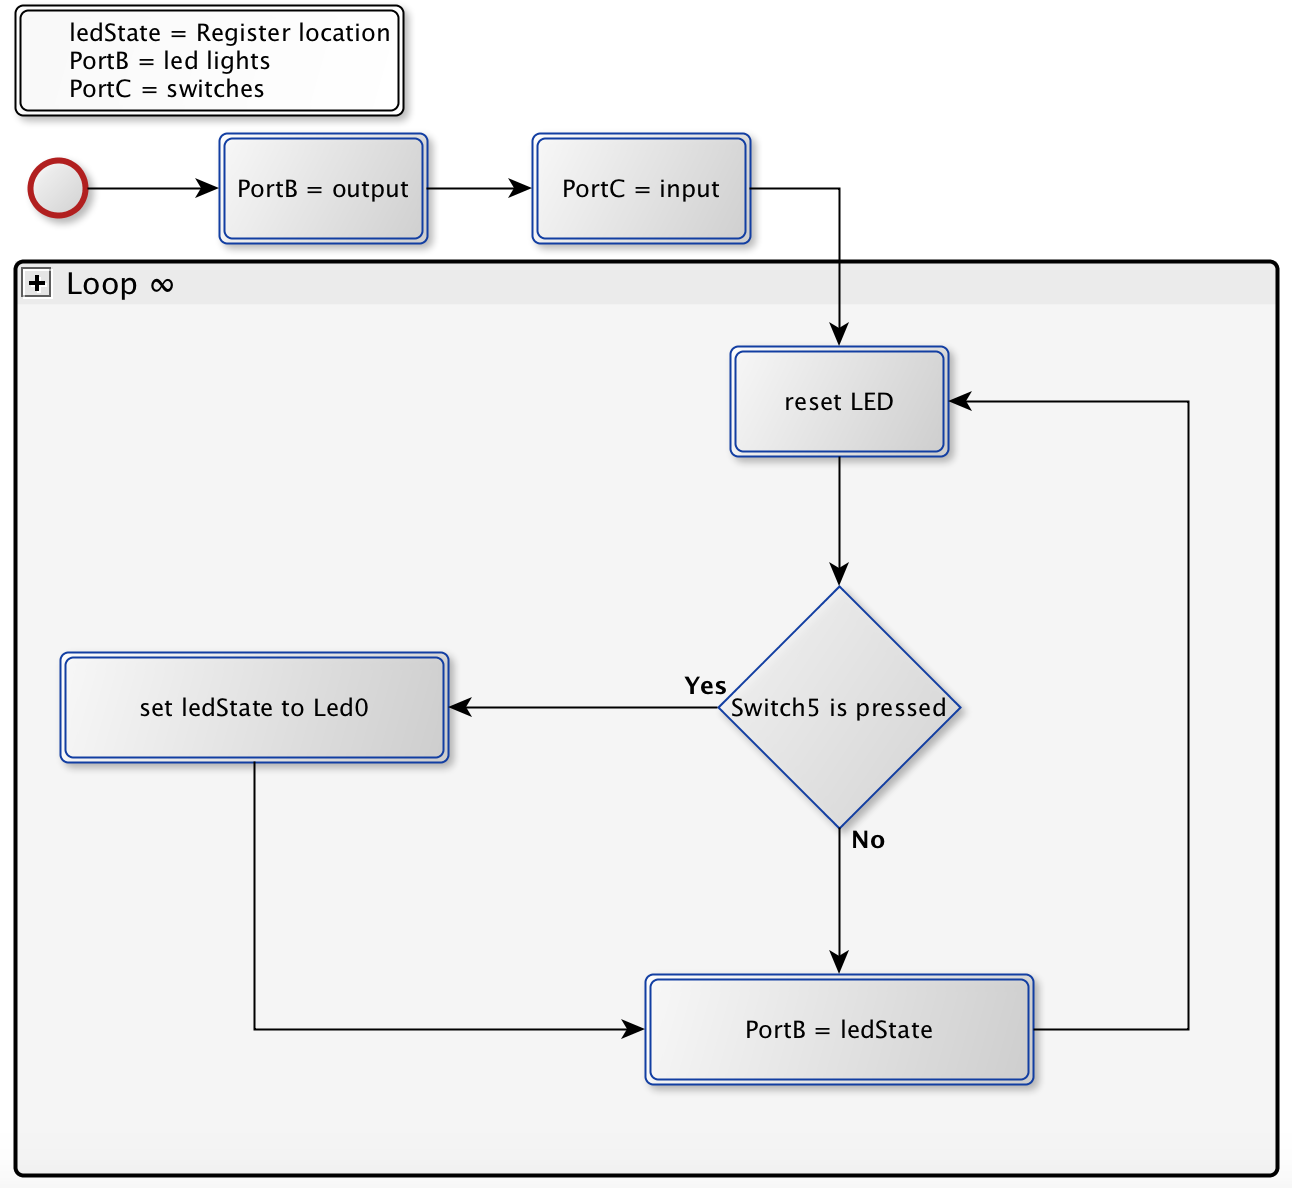
\includegraphics[scale=0.5]{Flowchart_pics/assignment3_pic.png} 
\caption{Flowchart}
\label{}
\end{figure}
\newpage
\subsection{Assembly Program}
\begin{lstlisting}[basicstyle=\tiny]
;>>>>>>>>>>>>>>>>>>>>>>>>>>>>>>>>>>>>>>>>>>>>>>>>>>>>>>>>>>>
;   1DT301, Computer Technology I
;   Date: 2017-09-04
;   Author:
;                       Caroline Nilsson            (cn222nd)
;                       Daniel Alm Grundstrom       (dg222dw)
;
;   Lab number:         1
;   Title:              How to use the PORTs. Digital input /output.
;                       Subroutine call.
;
;   Hardware:           STK600, CPU ATmega2560
;
;   Function:           Turns on LED0 when SW5 is held down.
;
;   Input ports:        PORTD
;
;   Output ports:       PORTB
;
;   Subroutines:        N/A
;   Included files:     m2560def.inc
;
;   Other information:  As with assignment 2, we have to keep in mind that
;                       a pressed switch is registered as a 0.
;
;   Changes in program: 
;                       2017-09-01:
;                       Implemented flowchart design.
;
;                       2017-09-04:
;                       Minor refactoring. Adds header and comments.
;
;<<<<<<<<<<<<<<<<<<<<<<<<<<<<<<<<<<<<<<<<<<<<<<<<<<<<<<<<<<<
.include "m2560def.inc"
.def dataDir = r16
.def ledState = r17

; Set PortB as output
ldi dataDir, 0xFF
out DDRB, dataDir

; Set PortD as input
ldi dataDir, 0x00
out DDRD, dataDir

loop:
    clr ledState                    ; Clear LED state so LED is turned off when
                                    ; button is released

    sbis PIND, PIND5                ; If SW5 is pressed down (PIND5 bit is zero)
        ldi ledState, 0x01          ;   then set LED0 state to turned on

    out PORTB, ledState             ; write state to LEDs
    rjmp loop

\end{lstlisting}
\newpage

\section{Assignment 4}
\begin{algorithm}
\begin{algorithmic}
\Procedure{Pseudocode}{}
\State{}
\EndProcedure
\caption{}
\label{}
\end{algorithmic}
\end{algorithm}

\begin{figure}[h]

\caption{Flowchart}
\label{}
\end{figure}

\subsection{Assembly Program}
\begin{lstlisting}

\end{lstlisting}
\newpage

\section{Assignment 5 - Waterfall}
\begin{algorithm}
\begin{algorithmic}
\Procedure{Pseudocode}{}
\State{$Initialize\ stack\ pointer$}
\State{$PortB = output$}
\State{$ledState = 1$} \Comment{$ledState = register\ location$}
\Repeat
\State{$ledState \rightarrow PortB$}
\State{$Delay\ 0.5\ sec$}
\If{$LED7\ is\ lit$}
\State{$ledState = 1$}
\EndIf
\If{$LED7\ is\ not\ lit$}
\State{$Move\ to\ left$}
\EndIf
\Until{$\infty$}
\EndProcedure
\caption{Waterfall simulation using LEDs}
\label{}
\end{algorithmic}
\end{algorithm}

\begin{figure}[h]
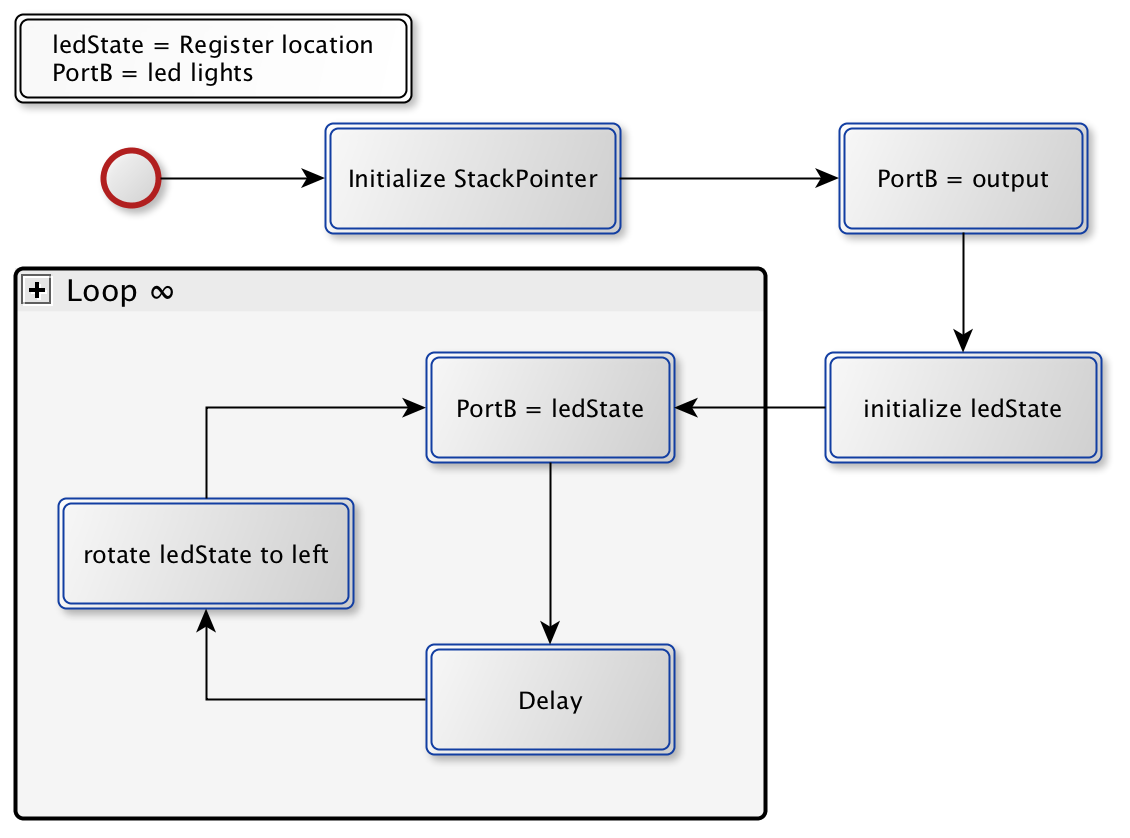
\includegraphics[scale=0.5]{Flowchart_pics/assignment5_pic.png} 
\caption{Flowchart}
\label{}
\end{figure}
\newpage
\subsection{Assembly Program}
\begin{lstlisting}[basicstyle=\tiny]
;>>>>>>>>>>>>>>>>>>>>>>>>>>>>>>>>>>>>>>>>>>>>>>>>>>>>>>>>>>>
;   1DT301, Computer Technology I
;   Date: 2017-09-04
;   Author:
;                       Caroline Nilsson            (cn222nd)
;                       Daniel Alm Grundstrom       (dg222dw)
;
;   Lab number:         1
;   Title:              How to use the PORTs. Digital input /output.
;                       Subroutine call.
;
;   Hardware:           STK600, CPU ATmega2560
;
;   Function:           Repeatedly lights LEDs sequentially right to left.
;                       
;                       I.e:
;                       0000 0001 -> 0000 0010 -> 0000 0100 -> ... ->
;                       1000 0000 -> 0000 0001 -> 0000 0010 -> ...
;
;   Input ports:        N/A
;
;   Output ports:       PORTB
;
;   Subroutines:        delay_500ms - delays execution for 500 ms
;   Included files:     m2560def.inc
;
;   Other information:  Since a subroutine is used, the stack pointer must
;                       be initialized so the processor knows where in the 
;                       code to jump when the subroutine returns. 
;
;   Changes in program: 
;                       2017-09-01:
;                       Implements flowchart design
;
;                       2017-09-04:
;                       Adds header, comments and some minor refactoring
;
;<<<<<<<<<<<<<<<<<<<<<<<<<<<<<<<<<<<<<<<<<<<<<<<<<<<<<<<<<<<
.include "m2560def.inc"
.def dataDir = r16
.def ledState = r17
.def INITIAL_LED_STATE = 0x01

; Initialize SP, Stack Pointer
ldi r20, HIGH(RAMEND)                   ; R20 = high part of RAMEND address
out SPH,R20                             ; SPH = high part of RAMEND address
ldi R20, low(RAMEND)                    ; R20 = low part of RAMEND address
out SPL,R20                             ; SPL = low part of RAMEND address

; Set PORTB to output
ldi dataDir, 0xFF
out DDRB, dataDir

ldi ledState, INITIAL_LED_STATE         ; Set initial LED state

loop:
    out PORTB, ledOutput                ; Write state to LEDs
    rcall delay_500ms                   ; Delay to make changes visible

    sbic PORTB, PORTB7                  ; If LED7 is lit
        ldi ledState, INITIAL_LED_STATE ;    then reset LED state to initial

    sbis PORTB, PORTB7                  ; else
        lsl ledState                    ;    shift LED state to the left 
    rjmp loop

; Generated by delay loop calculator
; at http://www.bretmulvey.com/avrdelay.html
;
; Delay 4 000 000 cycles
; 500ms at 8.0 MHz
delay_500ms:
    ldi  r18, 21
    ldi  r19, 75
    ldi  r21, 191
L1: dec  r21
    brne L1
    dec  r19
    brne L1
    dec  r18
    brne L1
    nop
    ret

\end{lstlisting}
\newpage

\section{Assignment 6 - Johnson counter}
\begin{algorithm}
\begin{algorithmic}
\Procedure{Pseudocode}{}
\State{$PortB = output$}
\State{$currentValue = 0$} \Comment{$currentValue = register\ location$}
\State{$multiplier = 2$} \Comment{$multiplier = register\ location$}
\Repeat \Comment{$Loop\_1\ (count\ up)$}
\If{$LED7\ is\ lit$}
\State{$Continue\ at\ Loop\_2$}
\Else
\State{$currentValue \times multiplier \rightarrow currentValue$}
\State{$Increase\ currentValue\ by\ 1$}
\EndIf
\State{$currentValue \rightarrow PortB$}
\State{$Delay\ 0.5\ sec$}
\Until{$\infty$}
\Repeat \Comment{$Loop\_2\ (count\ down)$}
\If{$LED0\ is\ lit$}
\State{$Continue\ at\ Loop\_1$}
\Else
\State{$Move\ right$}
\EndIf
\State{$currentValue \rightarrow PortB$}
\Until{$\infty$}
\EndProcedure
\caption{Johnson counter simulation using LEDs}
\label{}
\end{algorithmic}
\end{algorithm}

\begin{figure}[h!]
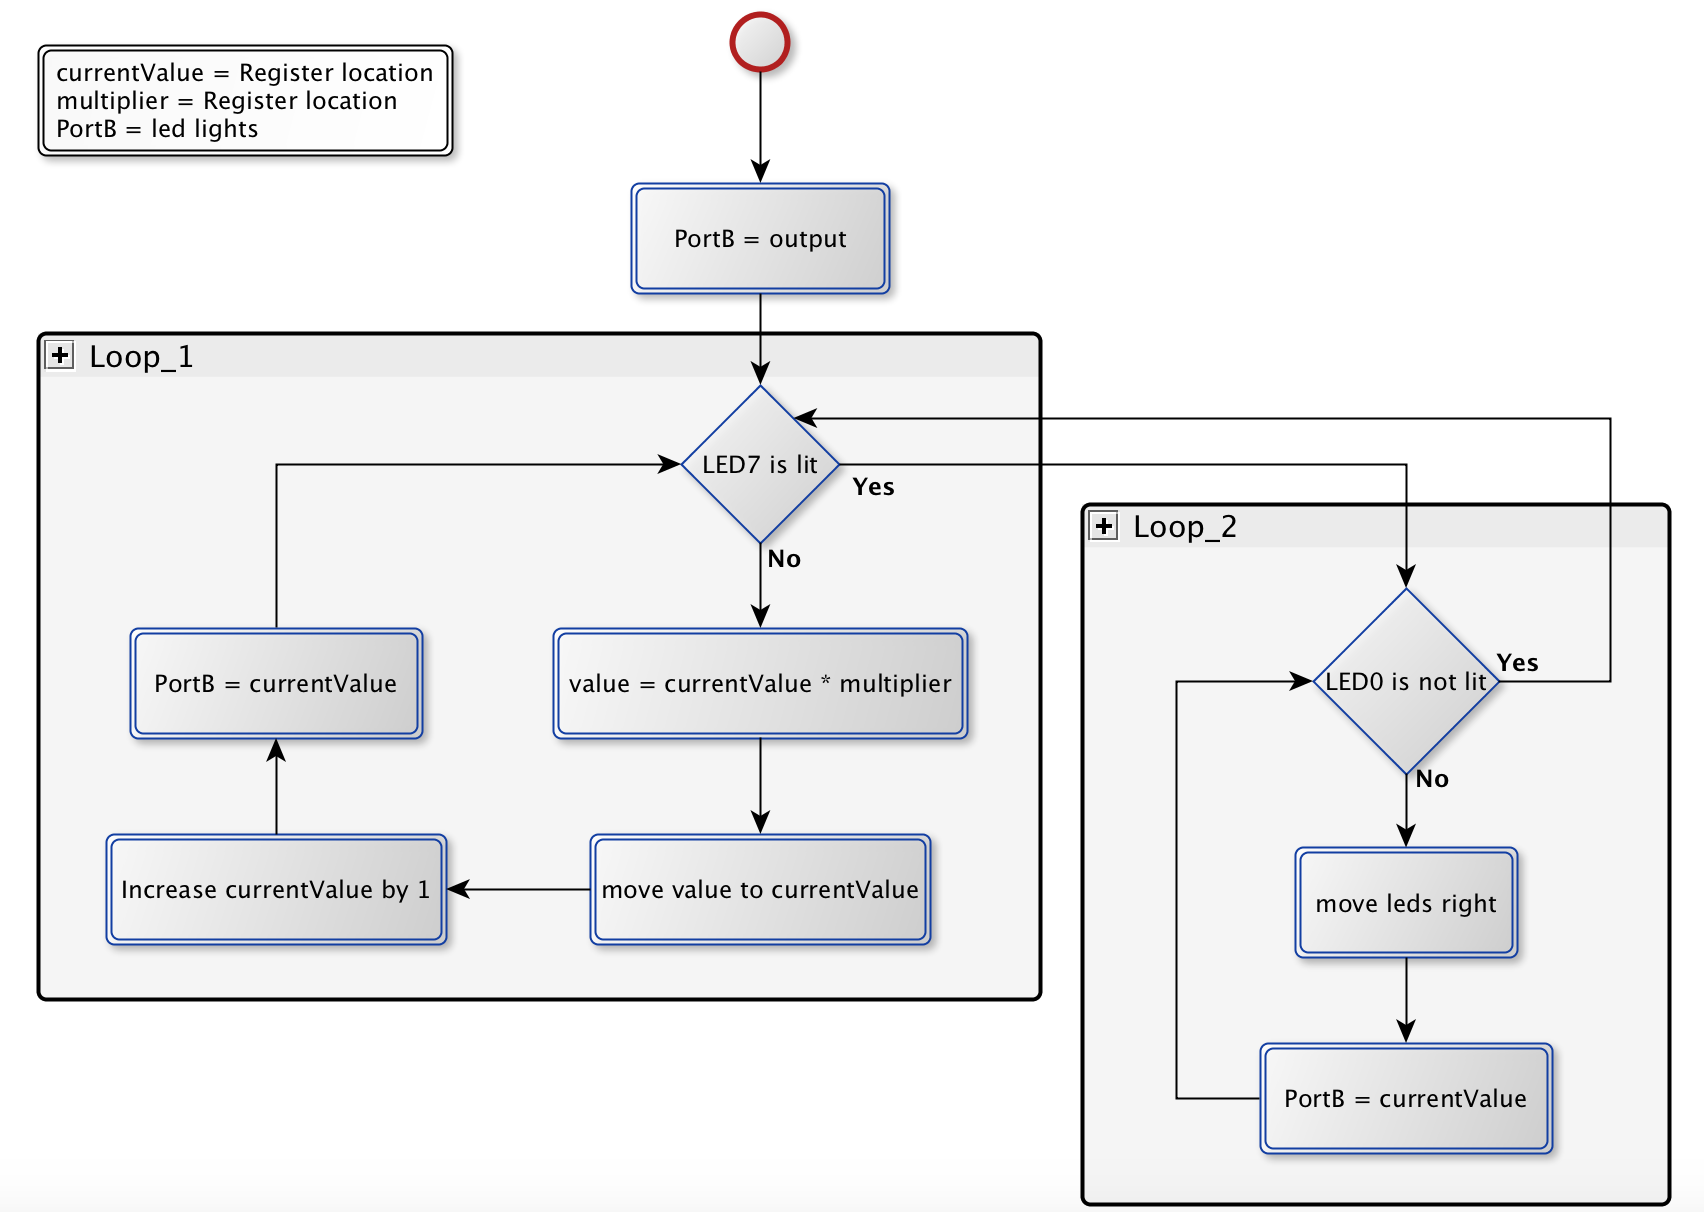
\includegraphics[scale=0.5]{Flowchart_pics/assignment6_pic.png} 
\caption{Flowchart}
\label{}
\end{figure}
\newpage
\subsection{Assembly Program}
\begin{lstlisting}[basicstyle=\tiny]
;>>>>>>>>>>>>>>>>>>>>>>>>>>>>>>>>>>>>>>>>>>>>>>>>>>>>>>>>>>>
;   1DT301, Computer Technology I
;   Date: 2017-09-04
;   Author:
;                       Caroline Nilsson            (cn222nd)
;                       Daniel Alm Grundstrom       (dg222dw)
;
;   Lab number:         1
;   Title:              How to use the PORTs. Digital input /output.
;                       Subroutine call.
;
;   Hardware:           STK600, CPU ATmega2560
;
;   Function:           Lights LEDs as a Johnson counter in an infinite loop. 
;
;                       I.e:
;                       0000 0001 -> 0000 0011 -> 0000 0111 -> ...
;                       1111 1111 -> 0111 1111 -> 0011 1111 -> ...
;
;   Input ports:        N/A
;
;   Output ports:       PORTB
;
;   Subroutines:        count_up - Counts the Johnson counter up
;                       count_down - Counts the Johnson counter down
;                       delay_500ms - delay execution for 500 ms
;
;   Included files:     m2560def.inc
;
;   Other information:  N/A
;
;   Changes in program: 
;                       2017-09-02:
;                       Implements flowchart design
;
;                       2017-09-04:
;                       Adds header and comments
;
;<<<<<<<<<<<<<<<<<<<<<<<<<<<<<<<<<<<<<<<<<<<<<<<<<<<<<<<<<<<
.include "m2560def.inc"
.def dataDir = r16
.def currentValue = r17                 ; Current value of Johnson counter
.def multiplier = r18

; Initialize SP, Stack Pointer
ldi r20, HIGH(RAMEND)                   ; R20 = high part of RAMEND address
out SPH,R20                             ; SPH = high part of RAMEND address
ldi R20, low(RAMEND)                    ; R20 = low part of RAMEND address
out SPL,R20                             ; SPL = low part of RAMEND address

ldi currentValue, 0x00
ldi multiplier, 0x02

; Set PORTB as output
ldi dataDir, 0xFF
out DDRB, dataDir

count_up:
    sbic PORTB, PORTB7                  ; If LED7 is lit (i.e. all LEDs lit)
        rjmp count_down                 ;   then start counting down

    ; Get next johnson value by multiplying by 2 and adding 1
    mul currentValue, multiplier
    mov currentValue, r0
    inc currentValue

    out PORTB, currentValue             ; Ouput johnson value to LEDs
    rcall delay_500ms                   ; Delay to make changes visible
    rjmp count_up                       ; Continue counting up

count_down:
    sbis PORTB, PORTB0                  ; If LED0 is unlit (i.e. all LEDs unlit)
        rjmp count_up                   ;   then start counting up

    lsr currentValue                    ; Shift to right to get previous
                                        ; johnson value

    out PORTB, currentValue             ; Output johnson value to LEDs
    rcall delay_500ms                   ; Delay to make changes visible
    rjmp count_down                     ; Continue counting down

; Generated by delay loop calculator
; at http://www.bretmulvey.com/avrdelay.html
;
; Delay 4 000 000 cycles
; 500ms at 8.0 MHz
delay_500ms:
    ldi  r31, 21
    ldi  r30, 75
    ldi  r29, 191
L1: dec  r29
    brne L1
    dec  r30
    brne L1
    dec  r31
    brne L1
    nop
    ret

\end{lstlisting}


\end{document}